% Author : Alain Matthes
% Encoding : UTF8
% Engine : PDFLaTeX
\documentclass[]{article}
\usepackage[utf8]{inputenc} 
\usepackage[usenames,dvipsnames]{xcolor}
\usepackage{fullpage}
\usepackage[upright]{fourier}
\usepackage{tkz-berge}
\thispagestyle{empty}
\begin{document}
\SetVertexSimple
\SetVertexNoLabel
\begin{center}
 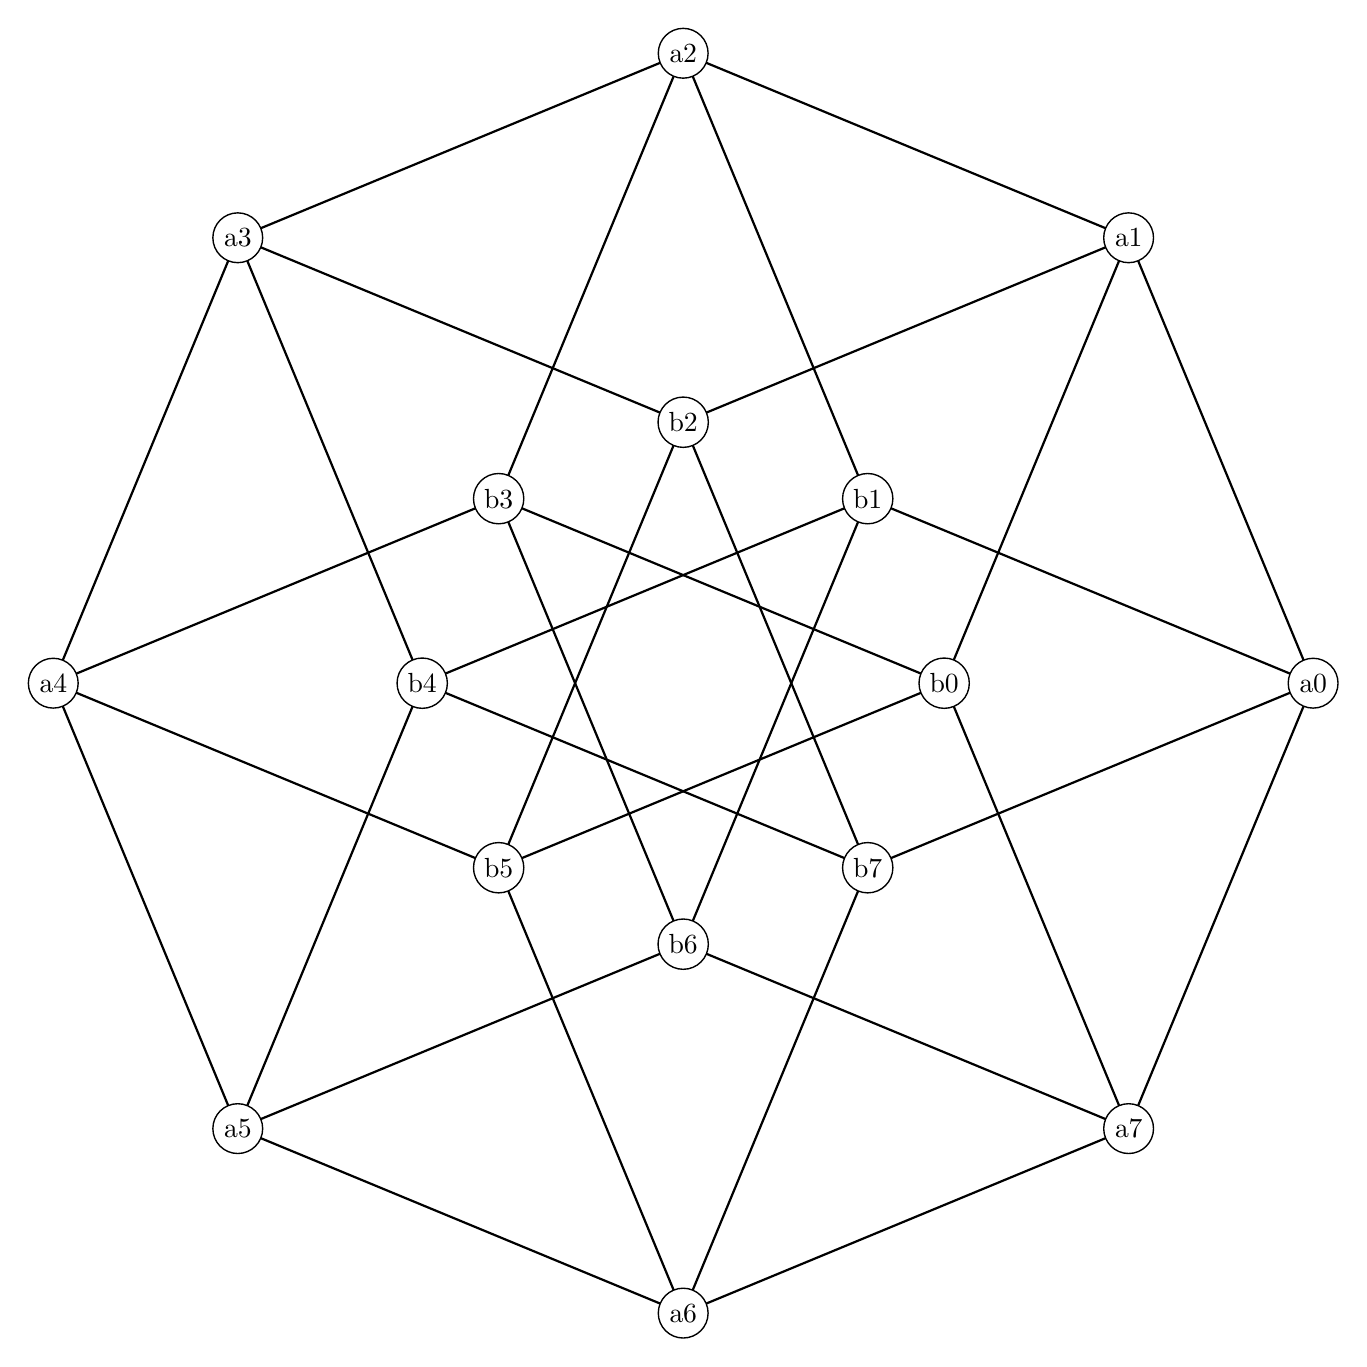
\begin{tikzpicture}
   \grCycle[RA=8]{8}
   \pgfmathparse{8*(1-4*sin(22.5)*sin(22.5))}
   \let\tkzbradius\pgfmathresult
   \grCirculant[prefix=b,RA=\tkzbradius]{8}{3}
\makeatletter
   \foreach \vx in {0,...,7}{%
     \pgfmathsetcounter{tkz@gr@n}{mod(\vx+1,8)}
     \pgfmathsetcounter{tkz@gr@a}{mod(\vx+7,8)}
     \pgfmathsetcounter{tkz@gr@b}{mod(\thetkz@gr@n+1,8)}
     \Edge(a\thetkz@gr@n)(b\thetkz@gr@b)
     \Edge(b\thetkz@gr@a)(a\vx)
      }
\makeatother
\end{tikzpicture}
\end{center}

\end{document}